% % % % % % % % % % % % % % % % % % % % % %
%
%	PREAMBLE
%
% % % % % % % % % % % % % % % % % % % % % %

% PAGE STYLE SETTINGS
	%\documentclass[12pt, oneside, a4paper]{art}		% PDF report style
	\documentclass[12pt, oneside, a4paper]{article}		% PDF article style
	%\documentclass[12pt, twoside, a4paper]{report}		% book style

% PACKAGES SETTINGS
	\usepackage[T1]{fontenc} 							% encoding input T1 codec
	\usepackage[utf8]{inputenc}							% encoding output
	\usepackage[ngerman]{babel}							% language settings German
	%\usepackage[english]{babel}						% language settings English
	\usepackage{fancyhdr}								% custom header and footer
	\usepackage{lastpage}								% label (variable) {LastPage}
	\usepackage[square,sort,comma,numbers]{natbib}		% reference style
	\usepackage{cite}									% citations
	\usepackage{listings}								% integration of listings
	\usepackage{graphicx}								% integration of graphics
	\usepackage{blindtext}								% generate bt with \blindtext or \blindtext[AMOUNT]
	\usepackage{microtype}								% justification
	\usepackage{lettrine}								% initial letter big
	\usepackage{multicol}								% multi column
	\usepackage{float}									% for graphics with caption
	\usepackage{seqsplit}								% for breaks in long titles
	\usepackage[a4paper, bindingoffset=.508cm, left=2.54cm, right=2.54cm, top=2.54cm, bottom=2.54cm, footskip=.63cm]{geometry}												% for customized margins

% FONTS SETTINGS
	%\usepackage[sfdefault]{cabin}						% default font
	%\usepackage[default]{droidserif}					% default font
	\usepackage{courier}								% font for listings


% HEADER AND FOOTER SETTINGS
	\setlength{\headheight}{0.5291cm}
	\renewcommand{\headrulewidth}{0.01cm}
	\pagestyle{fancy}
	\lhead{\insertauthor}								% top left
	\chead{}											% top center
	\rhead{\inserttitle}								% top right
	\lfoot{August 2015}									% bottom left
	\cfoot{}											% bottom center
	\rfoot{\thepage}									% bottom right
	%\rfoot{Page \thepage \ of \pageref{LastPage}}		% bottom right

% LISTINGS SETTINGS
	\lstset{
		basicstyle=\footnotesize\ttfamily,  			% set font Courier
		captionpos=b, 									% description under listings
		xleftmargin=0.5cm								% indent listing block
	}

% REFERENCES SETTINGS
	\addto\captionsenglish{\renewcommand{\refname}{References}}
	\bibliographystyle{plain}							% bib style

% TITLE SETTINGS										
	\title{ZIMG}
	\author{Christian Pleines, Stefan Bieliauskas, Fabian Junge, Oke Schwien}
	\date{2015 08 10}

\makeatletter
\renewcommand{\maketitle}{\bgroup\setlength{\parindent}{0pt}
	\begin{center}
		\vspace{4cm}
  		\seqsplit{\Huge{\textbf{\inserttitle}}}

  		\vspace{0.4cm}
  		\Large{Das Imageboard für's ZIMT}

  		\vspace{2cm}
  		\small{entstanden im Rahmen des Moduls \textit{Datenbankbasierte Web-Anwendungen} im Sommersemester 2015}

  		\vspace{2cm}
  		\large{\insertauthor}

  		\vspace{8cm}
  		\small{\insertdate}

  		\small{Hochschule Bremen -- City University of Applied Sciences}

	\end{center}\egroup
}

\let\inserttitle\@title

\let\insertauthor\@author

\let\insertdate\@date

\makeatother

% TEXT SETTINGS
	\setlength{\columnsep}{0.8818cm}					% column seperation
	\setlength{\parindent}{0cm}							% indentation off -> 0cm

% % % % % % % % % % % % % % % % % % % % % %
%
%	DOCUMENT
%
% % % % % % % % % % % % % % % % % % % % % %

\begin{document}

% TITLE
\begin{figure}[H]
	\centering
 	
\includegraphics[width=6cm]{footage/Hochschule_Bremen_Logo_RGB} 
	\label{logoofhochschulebremengermany}
\end{figure}

\maketitle												% print default title
\thispagestyle{empty}									% disable page numbers

\newpage

% INHALTSVERZEICHNIS
\tableofcontents
%\thispagestyle{empty}									% disable page numbers

\newpage

% TEXT
\section{Spezifikation}
% 1 Spezifikation
% In diesem Kapitel sollen die folgenden Punkte erläutert werden:
% 	- Was leistet die Webanwendung?
%	- Welchen Mehrwert bietet die Webanwendung für dessen Nutzer?

Im Rahmen des Moduls Datenbankbasierte Web-Anwedungen an der Hochschule Bremen im Sommersemester 2015 bei Steve Liedtke entstand das Web-Imageboard ZIMG. ZIMG ist eine Plattform zum Betrachten von Bildern und Gifs über das Internet. Zur Zielgruppe für diese Plattform gehören diejenigen Studierenden, die der Fakultät 4 angehören und den Standort ZIMT (Zentrum für Informatik und Medientechnologien) der Hochschule Bremen besuchen. \\
Die Studierenden können sich einloggen, Bilder auf ZIMG hochladen und diese so mit der Community rund um ZIMG teilen. Zusätzlich können hochgeladene Bilder von den Benutzern favorisiert (bewertet), durch Tags kategorisiert und kommentiert werden. \\
ZIMG bietet außerdem die Möglichkeit die Top Ten Tags, Top Ten Bilder und Top Five User zu begutachten. \\
Diese Funktionen machen ZIMG zu einem Ort des Austausches zwischen Studierenden, die beispielsweise ihre Erlebnisse im Semester oder Auslandssemester mit ihren Kommilitonen teilen wollen.

\subsection{Anforderungen}
% 1.1 Anforderungen
% In diesem Unterkapitel sollen die vorgesehenen und die tatsächlich umgesetzten Anforderungen beschrieben und mit Hilfe von Use-Case- und Aktivitätsdiagrammen konkretisiert werden.

Die für ZIMG vorgesehenen User Anforderungen waren folgende (vgl. Abb. \ref{ZIMGUseCaseDiagram}):

\begin{itemize}
	\item Als User möchte ich Bilder auf die Imageboardplattform hochladen, um diese teilen zu können.
	\item Als User möchte ich Bilder markieren, um diese meinen Favoriten hinzuzufügen.
	\item Als User möchte ich Bilder mit Schlagworten versehen, um diese zu kategorisieren.
	\item Als User möchte ich Bilder mit einem Punktesystem bewerten können, um Bilder in ihrer Beliebtheit zu steigern.
	\item Als User möchte ich Bilder kommentieren können, um meine Meinung zum Bild äußern zu können.
\end{itemize}

\begin{figure}[H]
 	\centering
 	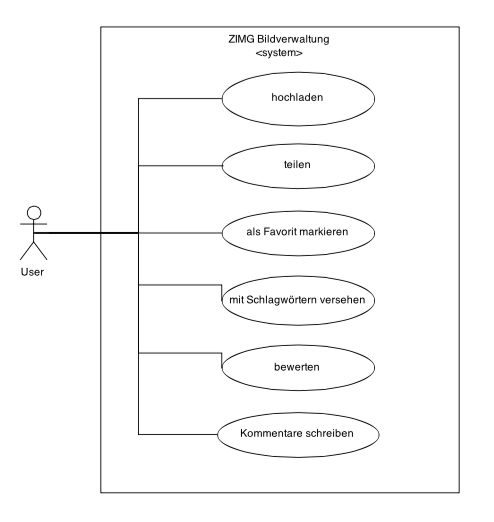
\includegraphics[width=8cm]{footage/ZIMG_UseCaseDiagram} 
 	\caption{ZIMG Use-Case-Diagramm}
	\label{ZIMGUseCaseDiagram}
 \end{figure}

 Es wurden alle Anforderungen an das System umgesetzt. Das bedeutet, dass ein eingeloggter User Bilder hochladen und somit teilen, Bilder favorisieren und somit bewerten, Bilder mit Schlagwörtern versehen (taggen) und Kommentare zu einzelnen Bildern verfassen kann.

\section{Architektur}
% 2 Architektur
% In diesem Kapitel soll beschrieben werden, wie das Projekt und die Datenbank strukturiert sind und welche Technologien und Frameworks verwendet werden.

\subsection{Gesamtarchitektur}
% 2.1 Gesamtarchitektur
% In diesem Unterkapitel soll beschrieben werden, wie die Gesamtarchitektur der entwickelten Webanwendung aussieht. Dies kann mit UML Paket- oder Klassendiagrammen unterstützt werden.

%\begin{figure}[H]
 %	\centering
 %	\includegraphics[width=\linewidth]{footage/ZIMG_Klassendiagramm} 
 %	\caption{ZIMG Klassendiagramm}
%	\label{ZIMGClassDiagram}
 %\end{figure}

\subsection{Programmabläufe}
% 2.2 Programmabläufe
% In diesem Unterkapitel sollte exemplarisch gezeigt werden, wie die typischen Abläufe in der Webanwendung aussehen. Hierfür sollten Aktivitäts-/Sequenzdiagramme genutzt werden.
\blindtext

\subsection{Persistenz}
% 2.3 Persistenz
% In diesem Unterkapitel soll die genutzte Datenbank und der Zugriff auf ihre Daten erläutert werden.
\blindtext

\subsubsection{Konzeption}
% 2.3.1 Konzeption
% In diesem Unterkapitel soll die konzipierte Datenbank nach ER-Diagramm beschrieben werden
\blindtext

\subsubsection{Umsetzung}
% 2.3.2 Umsetzung
% In diesem Unterkapitel soll die Datenbank nach relationalem Modell beschrieben werden. Außerdem sollten anwendungsspezifische Constraints aufgelistet werden, die bei der Implementierung bedacht werden müssen.
\blindtext

\subsubsection{Zugriff}
% 2.3.3 Zugriff
% In diesem Unterkapitel soll beschrieben werden mit welchen Technologien und Frameworks von der Webanwendung auf die Datenbank zugegriffen wird.
\blindtext

\subsection{Präsentation}
% 2.4 Präsentation
% In diesem Unterkapitel soll die Präsentationsschicht der Webanwendung beschrieben werden. Hierzu u.a. die genutzte Technologie/Framework. 
\blindtext

\newpage

\section{Installation}
% 3 Installation
% In diesem Kapitel soll beschrieben werden, welche Programmierwerkzeuge verwendet wurden und wie die Webanwendung lokal aufgesetzt werden kann

%Um am Projekt ZIMG strukturiert zusammen arbeiten zu können wurden folgende Tools genutzt, die ein verteiltes, aber weiterhin effizientes Arbeiten ermöglichen:

%\begin{description}
%	\item[Git] Die Versionsverwaltungssoftware wird genutzt, um u. a. den Source-Code auf dem Filehostingdienst Github in einem privaten Repository zu teilen und zu sichern
%	\item[Gradle] Als Build-Management-Automatisierungstool wird Gradle verwendet, um das Bauen des Projekts simpler zu gestalten
%	\item[Vagrant] Vagrant dient zur Erstellung einer separierten Entwicklungsumgebung, indem es eine lokale, virtuelle Maschine (eine Box) erstellt, die eine vorkonfiguerierte Testumgebung für die Entwicklung und darin enthaltene Infrastruktur-Komponenten (bspw. eine Datenbank) bereitstellt
%\end{description}

\subsection{Programmierwerkzeuge}
% 3.1 Programmierwerkzeuge
% Auflistung der verwendeten Programmierwerkzeuge mit Vor- und Nachteilen

Folgende Programmierwerkzeuge wurden unter Berücksichtigung ihrer Vor- und Nachteile eingesetzt, um für sie bestimmte Aufgaben zu erfüllen:

\begin{table}[ht!]
\centering
\begin{tabular}{| p{1.9cm} | p{6.2cm} | p{6.2cm} | l}
\hline                       
\textbf{Werkzeug}	& \textbf{Vorteile}	& \textbf{Nachteile}	\\
\hline
IntelliJ	& Schnelle Autovervollständigung, Übersichtlich, viele Shortcut-Funktionen, positive Erfahrung mit IntelliJ war vorhanden	& weniger verfügbare Plug-Ins als bspw. bei Eclipse vorhanden, unterstützt in der kostenfreien Version weniger Sprachen	\\
\hline
Vagrant	& Automatisiert den Entwicklungsumgebungserstellungsprozess und vereinfacht dadurch verteiltes Arbeiten	& Extra Einarbeitungs- und Konfigurationsphase	\\
\hline
Git	& lokal und somit schnell, vereinfacht dezentrale Zusammenarbeit via Internet, Sicherung der Daten durch Remote-Repository auf Filehostingdienst Github	& Extra Konfigurationsphase	(ware jedoch sehr kurz, da gute Kenntinsse im Team vorhanden)	\\
\hline
Jetty	& Geringe Größe, einfache Architektur, Einbindung ohne benötigten Webcontainer & Nicht so verbreitet wie TomCat	\\
\hline
MySQL	& Weit Verbreitet, unterstützt gängige Plattformen	& Bei Plattformen, die mehr Skalierbarkeit erfordern und bei der sehr große Datenmengen verwaltet werden müssen, bieten andere Datenbankensysteme mit nicht-relationalen Ansätzen (NoSQL) eventuell mehr Performance \\
\hline
Gradle	& Baut nur die veränderten Teile der Software, zum Großteil konfigurierbar	& Oft sind im Vergleich zu Maven keine definitiven Vorteile zu erkennen	\\
\hline
Hibernate	& Starke Abgrenzung von Präsentationsschicht vom Datenzugriff, Vereinfachung auf Datenzugriff, macht Datenbanksystem leicht austauschbar	& Extra Einarbeitungsphase \\
\hline
Spring	& Gute Objektverwaltung in Programmlogik, wenn einmal korrekt implementiert bietet Spring eine simple Nutzungstruktur	& Für kleine Projekte sehr groß und komplex \\
\hline
\end{tabular}
\caption{Programmierwerkzeuge mit Vor- und Nachteilen}
\label{ProgrammierwerkzeugeMitVorUndNachteilen}
\end{table}

\newpage

\subsection{Installation der Entwicklungsumgebung}
% 3.2 Installation der Entwicklungsumgebung
% Detaillierte Erklärung welche Maßnahmen notwendig sind, um die Entwicklungsumgebung aufzusetzen, sodass an dem Projekt mitentwickelt werden kann 

Folgende Schritte müssen durchgeführt werden, um die komplette Entwicklungsumgebung aufzusetzen:

\begin{enumerate}
	\item Installation Java Development Kit (Version 1.8.0\_05)
	\item Installation Git (Version 1.9.3)
	\item Installation IntelliJ (Version 14.1.3)
	\item Installation VirtualBox (Version 4.3.26)
	\item Installation Vagrant (Version 1.7.2)
	\item Installation Gradle (Version 2.2)
	\item Das Github-Repository \textit{https://github.com/B-Stefan/ZIMG} forken (bzw. als Contributor hinzugefügt werden und das Repository einfach klonen und einen neuen Branch erstellen)
	\item Das geforkte (oder geklonte) Projekt in IntelliJ öffnen
\end{enumerate}

\subsection{Konfiguration der Datenbank}
% 3.4 Konfiguration der Datenbank
% Beschreibung welche Schritte durchgeführt werden müssen, um die Datenbank mitsamt ihrer Struktur und Beispieldaten auf einem lokalen System aufzusetzen

Um die Datenbank lokal aufzusetzen müssen folgende Schritte durchgeführt werden:

\begin{enumerate}
	\item Im Terminal in das geforkte Verzeichnis navigieren und mit \textit{vagrant up} die virtuelle Maschine, die die Datenbank enthält, starten/erstellen
\end{enumerate}

\subsection{Installation der Anwendung}
% 3.3 Installation der Anwendung
% Beschreibung wie die Anwendung auf dem lokalen Rechner gestartet werden kann 

Das lokale Starten der Web-Andwendung benötigt die Durchführung folgender Schritte:

\begin{enumerate}
	\item Im Terminal in das geforkte Verzeichnis navigieren und mit \textit{vagrant up} die virtuelle Maschine, die die Datenbank enthält, starten/erstellen
	\item In IntelliJ mithilfe von Gradle die Anwendung bauen und den Jetty-Server starten
	\item In einem Web-Browser folgende Adresse eingeben: localhost:8080/login
\end{enumerate}

\end{document}

% % % % % % % % % % % % % % % % % % % % % %
%	EXAMPLES
% % % % % % % % % % % % % % % % % % % % % %

% initial letter big, footnotes, dots
	% \lettrine[lines=2]{H}{}ello\footnote{Hello is a word and it is a nice word; in other languages hello means Hallo, Bonjour, Hoi, \ldots} you, here I am the god and you are the ant.

% different lists
	% \begin{itemize}
	% 	\item one item
	% 	\item another item
	% 	\begin{itemize}
	% 		\item one subitem
	% 		\item another subitem
	% 	\end{itemize}
	% \end{itemize}

	% \begin{description}
	%   \item[girls] Sabrina, Monica, Suzanne
	%   \item[boys] Peter, Jack, Will
	%   \item[animals] lion, elephant, monkey
	% \end{description}

	% \begin{itemize}
	% 	\item one item
	% 	\item another item
	% 	\begin{enumerate}
	% 		\item first subitem
	% 		\item second subitem
	% 	\end{enumerate}
	% \end{itemize}

% include dividers
	% \begin{flushleft}
	% 	\rule{\linewidth}{0.01cm}
	% \end{flushleft}

% include graphics with caption and label
	% \begin{figure}[H]
	% 	\centering
	% 	\includegraphics[width=\linewidth]{footage/Hochschule_Bremen_Logo} 
	% 	\caption{Logo of Hochschule Bremen, Germany}
	%	\label{logoofhochschulebremengermany}
	% \end{figure}
  % how to mention this graphic in text
	% texttextext (Fig. \ref{logoofhochschulebremengermany}) texttexttext.

% quotation -- leading quote
	% \begin{quote}
	% \centering Our goal is to design everything so it's beautifully simple. \\
	% -- Larry Page, Google's July 2013 Q2 earnings call
	% \end{quote}

% tabular
%	\begin{table}[h!]
%	\centering
%	\scalebox{1.0}{
%	\begin{tabular}{| p{4cm} | p{10.3cm} | l}
%	\hline                       
%	\textbf{Taste} 	& \textbf{Befehl}		\\
%	\hline
%	A				& Bewegt den SuperJumperMan nach links	\\
%	\hline
%	D				& Bewegt den SuperJumperMan nach rechts	\\
%	\hline
%	Leertaste		& Lässt den SuperJumperMan springen \\
%	\hline
%	Pfeiltaste Oben & Zoomt die Kamera herein \\
%	\hline
%	Pfeiltaste Unten & Zoomt die Kamera heraus \\
%	\hline
%	Pfeiltaste Links & Dreht die Kamera nach links \\
%	\hline
%	Pfeiltaste Rechts & Dreht die Kamera nach rechts \\
%	\hline
%	\end{tabular}
%	}
%	\caption{Steuerung von SuperJumperManSupreme}
%	\label{Steuerung}
%	\end{table}